\qquad O Shell Sort é um algoritmo de ordenação por comparação que pode ser
entendido como uma generalização do Insertion Sort. Em vez de comparar
e deslocar apenas elementos adjacentes desde o início, o Shell Sort
primeiro ordena, de forma aproximada, subconjuntos de elementos
espaçados por um intervalo (chamado de \textit{gap}), e vai reduzindo
progressivamente esse intervalo até chegar a 1 — quando o algoritmo se
comporta exatamente como um Insertion Sort tradicional, porém sobre um
vetor que já está quase ordenado, o que reduz drasticamente o número
de deslocamentos necessários nessa última etapa.

\qquad A implementação utilizada neste trabalho adota a sequência de
intervalos originalmente proposta por Donald Shell: o primeiro
intervalo é tamanho/2, e a cada passada o intervalo é dividido por 2
(divisão inteira), até chegar a 1. Para cada intervalo (gap), aplica-se
a lógica do Insertion Sort a cada um dos subvetores formados por
elementos espaçados de \textit{gap} posições entre si.

\qquad A seguir apresenta-se a implementação utilizada neste trabalho, em
C++, correspondente à função \texttt{ShellSort\_versao1}:

\begin{verbatim}
void ShellSort_versao1(int *vetor, int tamanho) {
    int chave, j;
    for (int gap = tamanho / 2; gap > 0; gap /= 2) {
        for (int i = gap; i < tamanho; i++) {
            chave = vetor[i];
            j = i - gap;
            while (j >= 0 && vetor[j] > chave) {
                vetor[j + gap] = vetor[j];
                j -= gap;
            }
            vetor[j + gap] = chave;
        }
    }
}
\end{verbatim}

\qquad A escolha da sequência de intervalos é um dos aspectos mais
estudados do Shell Sort, pois afeta diretamente sua complexidade de
pior caso — esse ponto é discutido em detalhes, com base em pesquisa
bibliográfica, na seção de análise de complexidade deste capítulo,
conforme solicitado no enunciado do trabalho. De forma geral, mesmo
utilizando a sequência mais simples (a original de Shell), o algoritmo
apresenta desempenho muito superior ao Insertion, Selection e Bubble
Sort na prática, para todos os tipos de entrada testados.

\subsection{Teste de Mesa Manual}

\qquad Nesta seção deve ser inserida a digitalização do teste de mesa
manual do Shell Sort, realizado à mão com um exemplo de entrada
diferente dos exemplos trabalhados em sala de aula, conforme exigido
pelo enunciado do trabalho. Substitua a imagem de exemplo abaixo pela
digitalização (foto ou escaneamento) do teste de mesa manuscrito.

\begin{figure}[htbp]
    \centering
    % Substitua o arquivo abaixo pela digitalizacao do teste de mesa manuscrito
    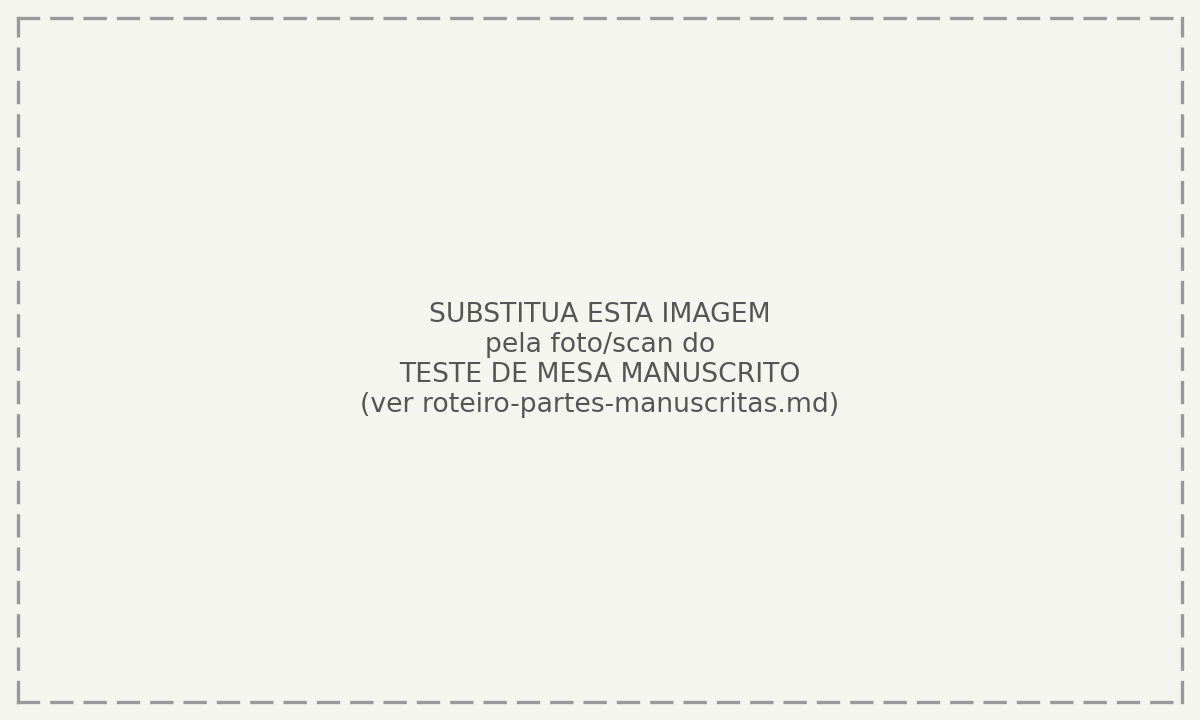
\includegraphics[width=14cm]{Imagens/Shell Sort/teste_de_mesa.png}
    \caption{Teste de mesa manual do algoritmo Shell Sort}
    \label{fig:teste_mesa_shell}
\end{figure}
